\chapter{Sperimentale}
\label{cha:Sperimentale}

\section{Ambiente}
\subsection{rete docker}
Per effettuare i test delle performance del reverse proxy é stato utilizzato un server sperimentale eseguito all'interno di un container docker. Per avviare tutti i servizi necessari per effettuare i test é stato creato un docker compose con le direttive per avviare il reverse proxy, il server di test e un'istanza di ubuntu da dove effettuare le richieste.

\begin{lstlisting}[language=DockerCompose]
version: "1.0"
services:
  reverse:
    build: .
    ports:
      - "8081:8081"
      - "8082:8082"
    volumes:
      - "./configuration_docker.json:/configuration.json"
      - "./reverse_proxy.com+3.pem:/reverse_proxy.com+3.pem"
      - "./reverse_proxy.com+3-key.pem:/reverse_proxy.com+3-key.pem"
      - "./log_file.log:/log_file.log"

  testserver:
    image: "kennethreitz/httpbin"
    ports:
      - "8080:80"

  ubuntu:
    container_name: ubuntu
    image: ubuntu
    restart: on-failure
    command: ["sleep","infinity"]

\end{lstlisting}

\subsection{httpbin}
\cite{httpbin}
Httpbin é un server con delle chiamate base che possono essere utilizzate per testare i propri dispositivi. Si possono quindi testare chiamate semplici come semplici \texttt{GET} e \texttt{POST} ma anche alcune piú complesse come chiamate per verificare il funzionamento dei cookies oppure per verificare i redirect. Di questo servizio esiste giá la versione containerizzata nello store di docker che quindi ha reso l'utilizzo immediato.

\subsection{ab}
\cite{ab}
\texttt{ab} é un comando incluso nel pacchetto \texttt{apache2-utils} che serve per fare test di carico nei server effettuando un numero di richieste http in sequenza.

\subsection{wireshark}
\cite{wireshark}
Wireshark é un software per analizzare il traffico passante per un porta di rete. Una volta dato l'accesso alla porta direte, wireshark mostra tutti i pacchetti tcp/udp che passano per quella porta. Quindi in questo caso si parla di protocolli di quarto livello.

\section{Elenco dei test}\label{test:settings}
Per verificare le performance del reverse proxy e valutare le differenze rispetto a una connessione diretta al servizio, sono stati effettuati test in quattro situazioni differenti.
\begin{enumerate}
  \item
    \begin{itemize}
      \item Reverse proxy: non collegato
      \item server: connesso tramite \texttt{http}
    \end{itemize}
  \item
    \begin{itemize}
      \item Reverse proxy: connesso tramite \texttt{http}
      \item server: connesso tramite \texttt{http}
    \end{itemize}
  \item
    \begin{itemize}
      \item Reverse proxy: connesso tramite \texttt{https}
      \item server: connesso tramite \texttt{http}
    \end{itemize}
\end{enumerate}
I fattori interessanti da valutare analizzando i risultati di questi test sono:
\begin{itemize}
  \item Quanta differeza di velocitá e grandezza dei pacchetti c'é tra una connessione non criptata e una criptata.
  \item Quanto differisce la velocitá di accesso alle risorse del server tra la connessione diretta e l'utilizzo di un reverse proxy.
\end{itemize}

\section{Procedura esecuzione test}
Per ognuna delle configurazioni definite precedentemente\ref{test:settings} vengono fatte 2 tipologie di test.
\begin{enumerate}
  \item
    \begin{itemize}
      \item Tramite il comando \texttt curl viene inviata una richiesta get al server all'indirizzo\\
        \texttt{\$ curl <URL>}
        \item Poi con wireshark si controlla quanti pacchetti sono stati inviati per effettuare lo scambio di dati

    \end{itemize}
  \item Tramite ab viene fatto un test a carico, cioé generando molte richieste e tenendo traccia del tempo impiegato per ultimarle e la dimensione totale dei pacchetti inviati. In questo caso vengono fatte 1000 richieste da 1 solo thread per ogni test.\\
    \texttt{\$ ab -n 1000 <URL>}

\end{enumerate}

\section{Risultati}
\subsection{Singola connessione}
In tabella sono riportati la quantitá di pacchetti scambiati e la dimensione totale di questi per una singola richiesta.
\begin{center}
  \begin{tabular}{|c|c|c|}
    \hline
    condizione & numero pacchetti & dimensione totale (bytes) \\
    \hline
    \hline
    http server & 14 & 9906 \\
    \hline
    http reverse proxy + http server & 14 + 12 = 26 & 9908 + 9961 = 19869 \\
    \hline
    https reverse proxy + http server & 27 + 14 = 41 & 12000 + 9961 = 21961 \\
    \hline
  \end{tabular}
\end{center}
\begin{center}
  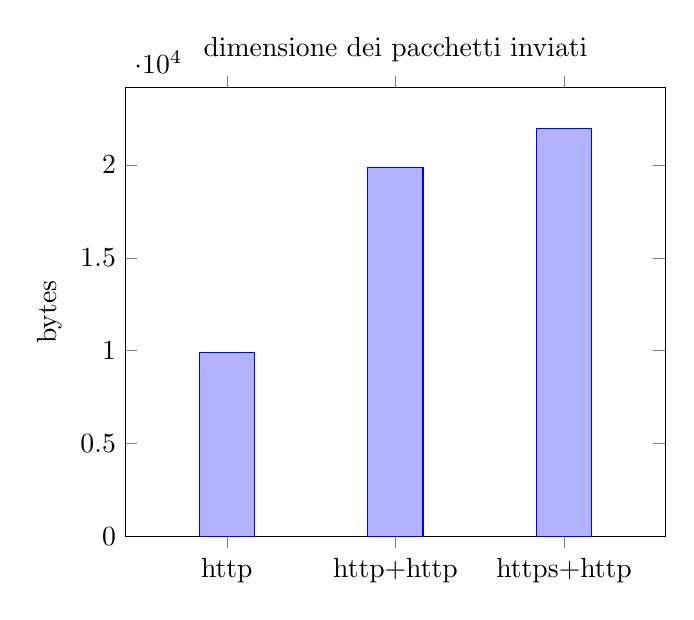
\begin{tikzpicture}
    \begin{axis}[
        ybar,
        title={dimensione dei pacchetti inviati},
        bar width=0.7cm,
        ylabel={bytes},
        symbolic x coords={http, http+http, https+http},
        xtick=data,
        enlarge x limits=0.3,
        ymin=0,
      ]
      \addplot
        coordinates {(https+http,21961) (http+http,19869) (http,9906)};
    \end{axis}
  \end{tikzpicture}
\end{center}


\subsection{1000 richieste}
In tabella é riportato il tempo impiegato per effettuare 1000 richiese in sequenza da signolo thread.
\begin{center}
  \begin{tabular}{|c|c|c|c|}
    \hline
    condizione & risultati (s) & media (s) & variazione standart (s) \\
    \hline
    \hline
    http server & \makecell {2.960 \\ 2.874 \\ 2.967} & 2.933 & 0.051 \\
    \hline
    http reverse proxy + http server & \makecell {4.539 \\ 4.521 \\ 4.512} & 4.524 & 0.014 \\
    \hline
    https reverse proxy + http server & \makecell {10.426 \\ 10.415 \\ 10.426} & 10.426 & 0.006 \\
    \hline
  \end{tabular}
\end{center}

\begin{center}
  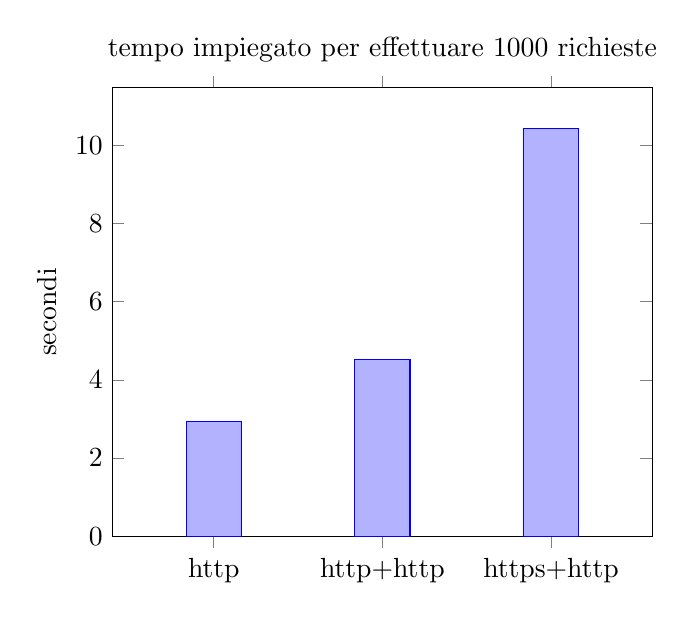
\begin{tikzpicture}
    \begin{axis}[
        ybar,
        bar width=0.7cm,
        title={tempo impiegato per effettuare 1000 richieste},
        ylabel={secondi},
        symbolic x coords={http, http+http, https+http},
        xtick=data,
        enlarge x limits=0.3,
        ymin=0,
      ]
      \addplot
        coordinates {(https+http,10.426) (http+http,4.524) (http,2.933)};
    \end{axis}
  \end{tikzpicture}
\end{center}

\subsection{Analisi risultati}
\subsubsection{Singola connessione}
Andando ad analizzare i risultati del test a singola connessione si possono vedere dei valore che ci si poteva aspettare considerando il funzionamento di un reverse proxy.
\begin{itemize}
  \item Prendendo in considerazione solamente la coppia \textbf{http e http + http} si puó notare che il risultato della seconda configurazione é praticamente doppio rispetto alla prima. Questo ce lo si poteva aspettare considerando il fatto che il reverse proxy non fa altro che copiare le richieste e le risposte inoltrandole all'altro nodo. Si possono vedere peró delle piccole differenze nella dimensione dei pacchetti tra il reverse proxy e il server. Questo é dovuto alla grandezza maggiore dell'header dovuta all'inserimento del campo \texttt{X-Forwarded-For}.
  \item Analizzando ora la coppia di risultati \textbf{http + http e https + http} si vede una differenza piccola e, facendo riferimento alla tabella, appartenente solamente allo scambio di pacchetti tra client e reverse proxy. Causa di questa differenza é il livella di sicurezza aggiunto alla connessione che necessita di scambiare informazioni per effettuare la criptazione dei dati. Come visto prima \ref{arte:handshake} per effettuare lo scambio in modo sicuro bisogna scambiare chiavi e concordarsi su alcune variabili. Questo processo fa si che la dimensione finale della connessione aumenti leggermente. Per richieste che implicano uno scambio di dati maggiore la differenza diminuisce visto che il processo viene fatto solo una volta.
\end{itemize}

\subsubsection{1000 richieste}
